\documentclass[11pt]{article}
\usepackage{graphicx, subfig}
\usepackage[top=1in, bottom=1in, left=1in, right=1in]{geometry}
\graphicspath{ {./figs/} }
\pagestyle{plain}
\begin{document}
\title{\vspace{-5mm}Voting Model and Edge Reconnecting Model CPI}
\author{Alexander Holiday}
\maketitle
\section*{Voting model}

Fig. \ref{fig:vmDynamics} reveals the correlations between conflicts and minority fractions in a single direct simulation. Similar correlations have been shown between the number of conflicting edges and the number of conflicting triangles (conflicting triangles are those in which one of the vertices has a different opinion than the other two). Fig. \ref{fig:vmPP} displays the phase-plane of the number of conflicts and the minority fraction. The initial, fast dynamics leading to the slow manifold are visible as the nearly-vertical lines leading to the curves. The number of conflicts quickly becomes a function of the minority fraction. All simulations were performed at an initial average degree of four, and an initially uniform distribution of opinions. The number of vertices varies from $200$ to $1,000$ in the figures below, but I wouldn't expect this to affect dynamics.

\begin{figure}[h!]
  \centering
  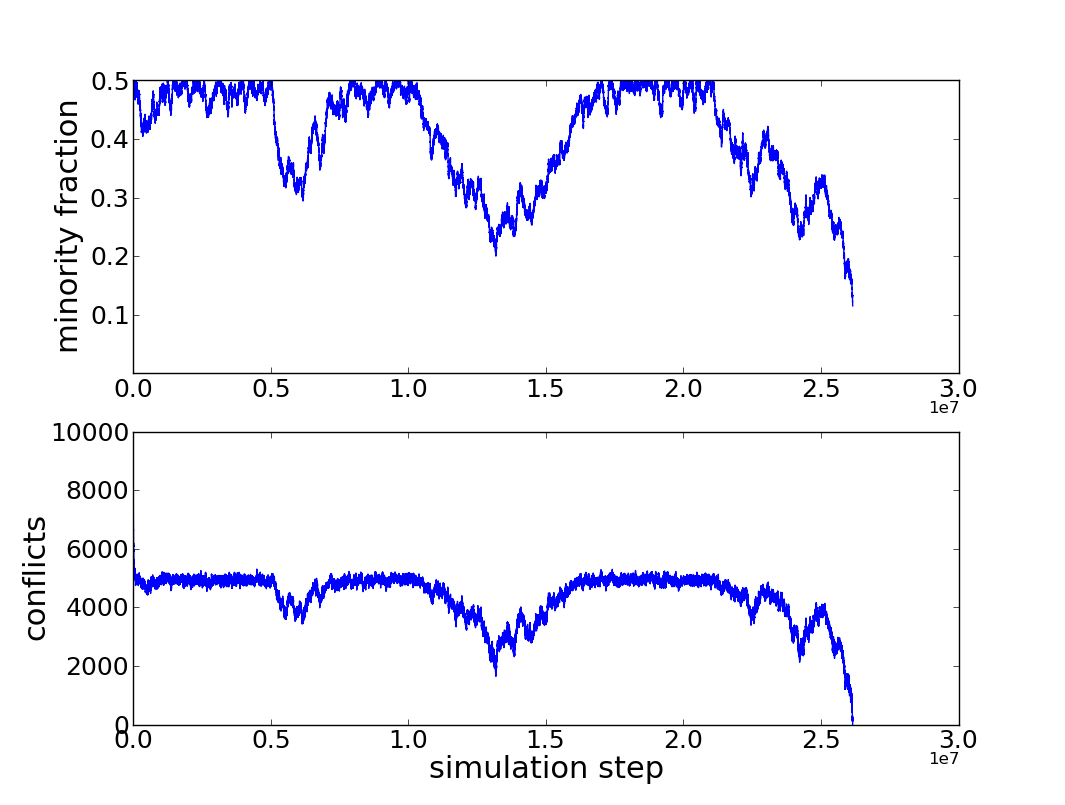
\includegraphics[height=100mm]{vmDynamics}
  \caption{Evolution of conflicts and minority fraction in a single voting model simulation.}
  \label{fig:vmDynamics}
\end{figure}

\begin{figure}[h!]
  \centering
  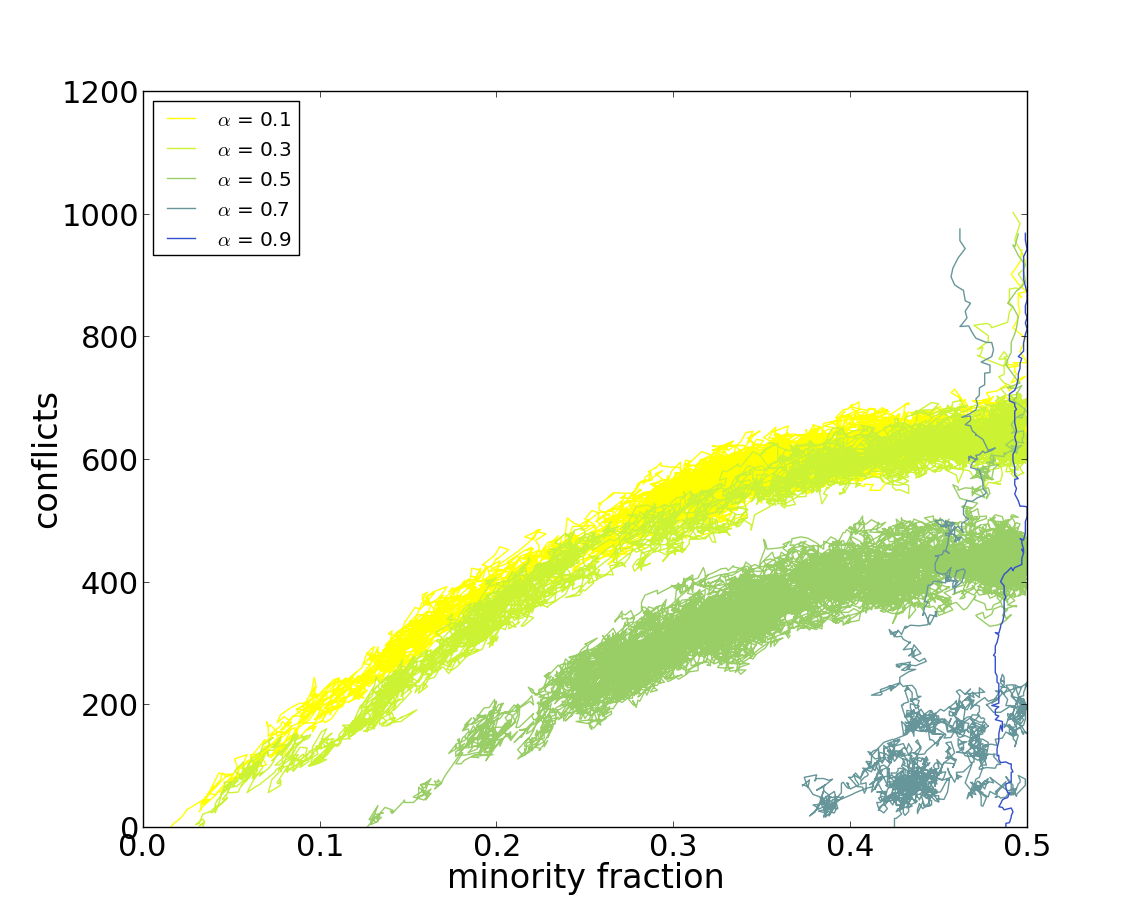
\includegraphics[height=90mm]{vmPhasePortrait}
  \caption{Phase portrait at varying values of $\alpha$.}
  \label{fig:vmPP}
\end{figure}

In Fig. \ref{fig:vmHealing}, the dark blue curve is the average evolution of $64$ direct simulations. The other curves were created using CPI with a projection step of zero, i.e. restricted and immediately lifted. They differ in the total number of direct simulation steps before this lift/restrict operation was performed. The red curve was simulated $5,000$ steps between lifting and restricting, the green $1,000$, and the light blue $15,000$. As the system is allowed more time to heal, it approaches the expected solution.

\begin{figure}[h!]
  \centering
  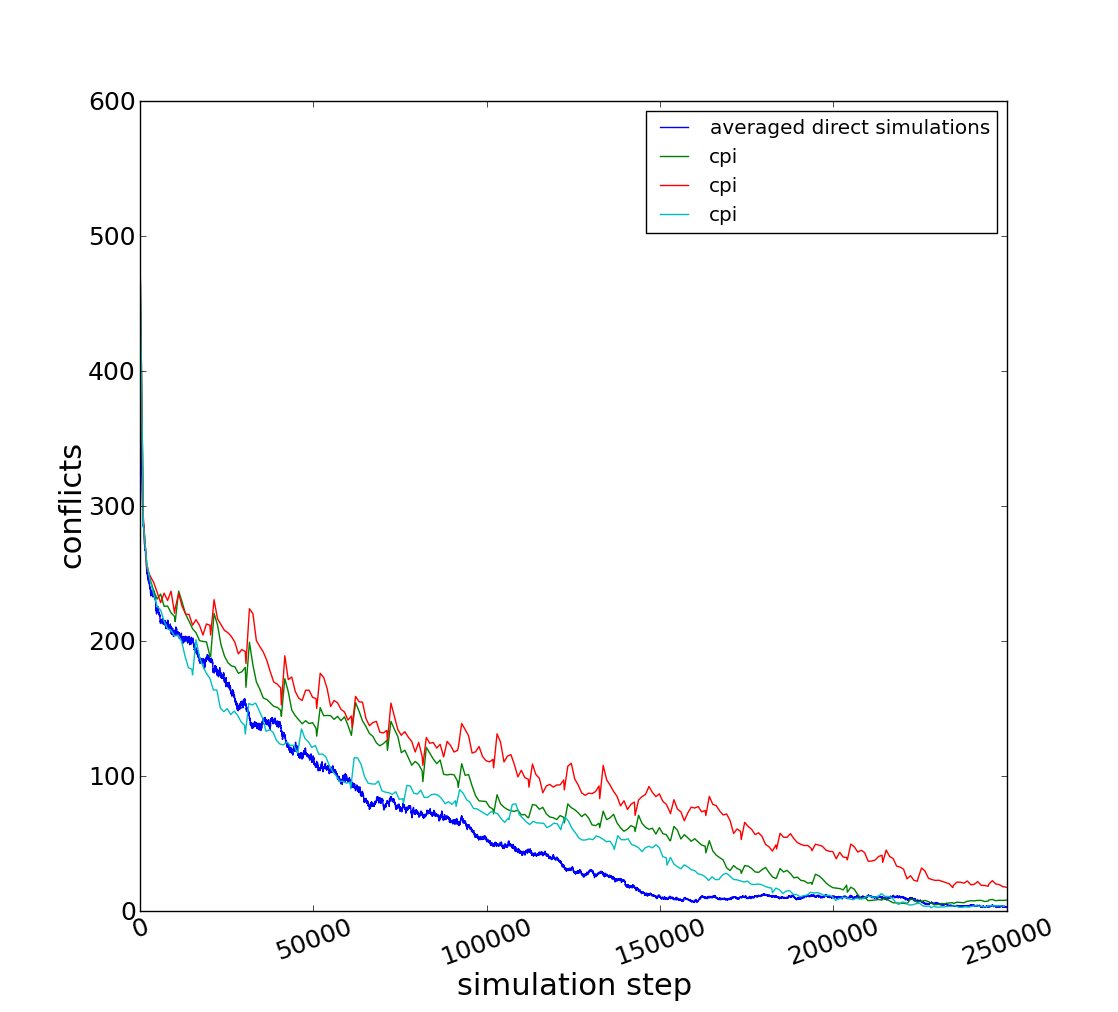
\includegraphics[height=100mm]{vmHealing}
  \caption{``Healing'' of voting model back to slow manifold, simulation was restricted and immediately lifted every $5,000$ to $15,0000$ steps.}
  \label{fig:vmHealing}
\end{figure}

The trajectories in Fig. \ref{fig:vmSlow} are taken from a CPI simulation in which an ensemble of eight trajectories was averaged to obtain a smoother evolution (though the figure presents each trajectory individually). In this scheme, eight voting models are initialized with the same conditions, and run, in this case, for $1,000$ direct simulation steps. After an initial healing period, here $200$ steps, the number of conflicts and the minority fraction, our course variables, are periodically collected from each model in the ensemble and averaged. This timecourse of averaged coarse evolution was then projected $200$ steps in conflict/minority fraction space. The ensemble was then initialized with this new number of conflicts and new minority fraction, and the process was repeated until all runs had converged. \\
\indent What separates Fig. \ref{fig:vmSlow} from Fig. \ref{fig:vmFast} is that in Fig. \ref{fig:vmSlow}, as soon as a run in the ensemble converged, i.e. reached zero conflicts, it was removed. Thus, as more and more models reached consensus, fewer and fewer were left in the CPI ensemble, creating more variability in averaged statistics. Alternatively, in Fig. \ref{fig:vmFast}, the statistics of these converged runs, i.e. a conflict count of zero and their final minority fraction, were averaged into the overall ensemble. This dragged the ensemble towards the consensus state of zero conflicts, and resulted in faster convergence. As an average of direct simulation trajectories would also record completed runs as zero conflict simulations, this second method seemed a truer representation of the macroscopic dynamics.\\
\indent Fig. \ref{fig:vmCPIPP} exhibits a jagged phase portrait from a CPI simulation that looks qualitatively like those from direct simulations, in Fig. \ref{fig:vmPP}.

\begin{figure}[h!]
  \centering
  \subfloat[Evolved $1000$ steps, projected $200$.]{
    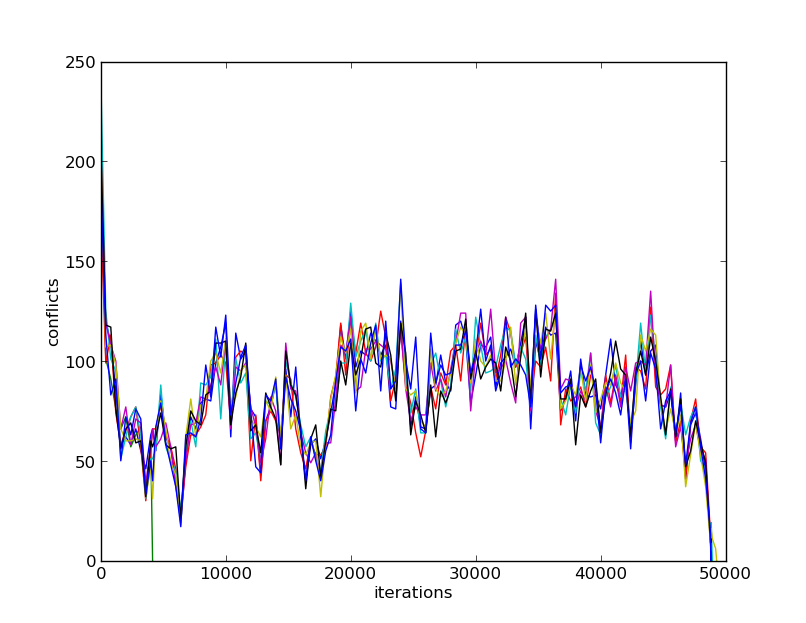
\includegraphics[height=100mm]{vmCPISlow1}
    \label{fig:vmSlow1}
  }
  \hspace{3mm}
  \subfloat[Evolved $1000$ steps, projected $200$.]{
    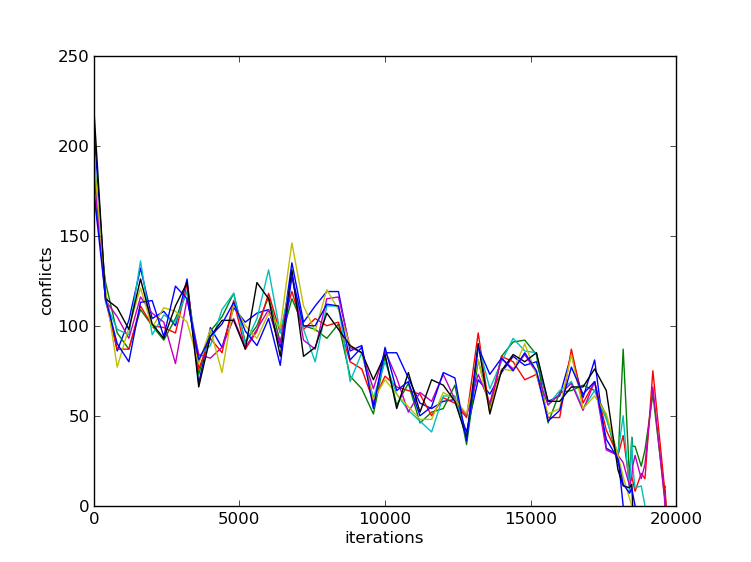
\includegraphics[height=100mm]{vmCPISlow2}
    \label{fig:vmSlow2}
  }
  \caption{First CPI method in which finished runs in the ensemble are entirely removed from the simulation. This causes slower convergence.}
  \label{fig:vmSlow}
\end{figure}

\begin{figure}[h!]
  \centering
  \subfloat[Evolved $15,000$ steps, projected $5,000$.]{
    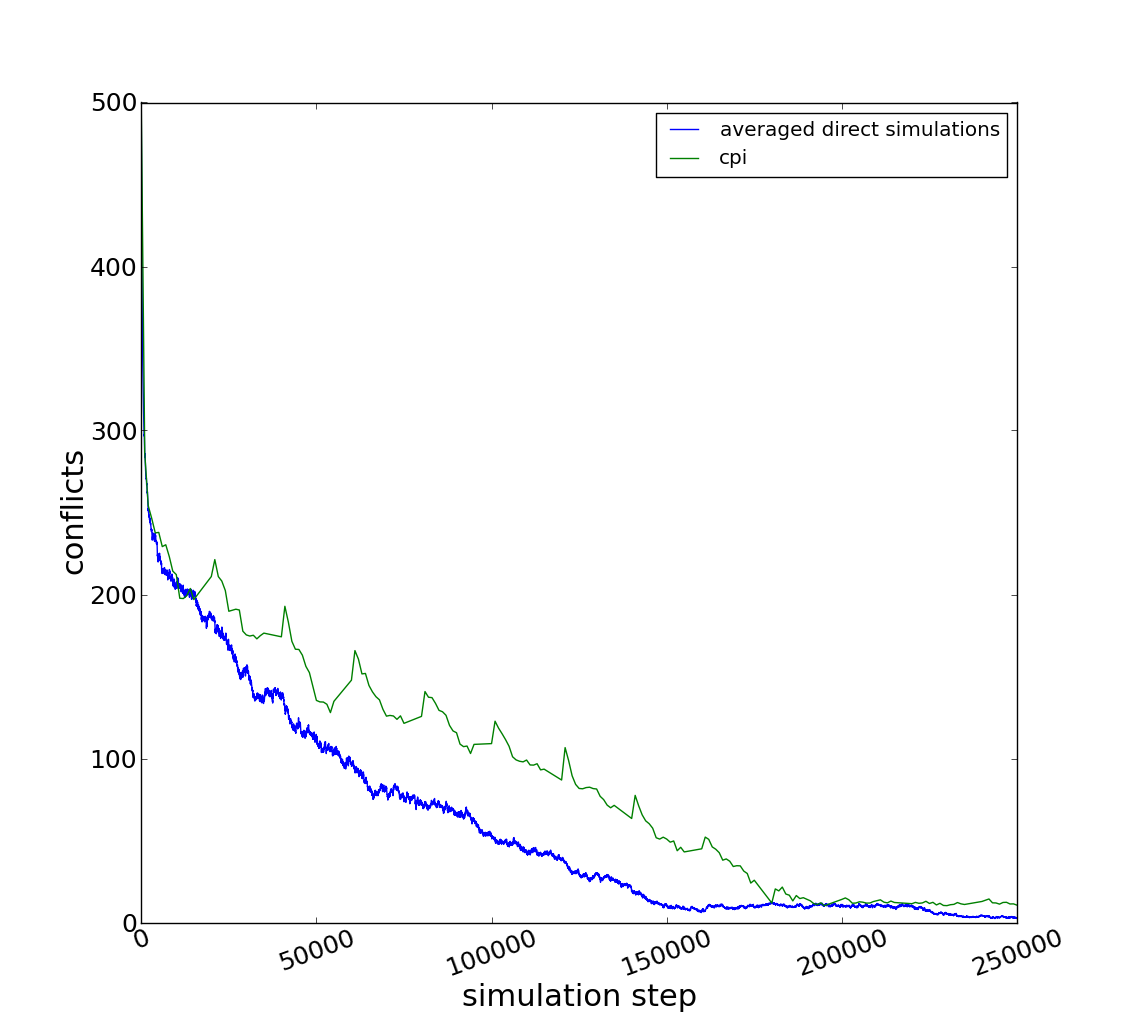
\includegraphics[height=65mm]{vmCPIFast1}
    \label{fig:vmFast1}
  }
  \hspace{3mm}
  \subfloat[Evolved $15,000$ steps, projected $10,000$.]{
    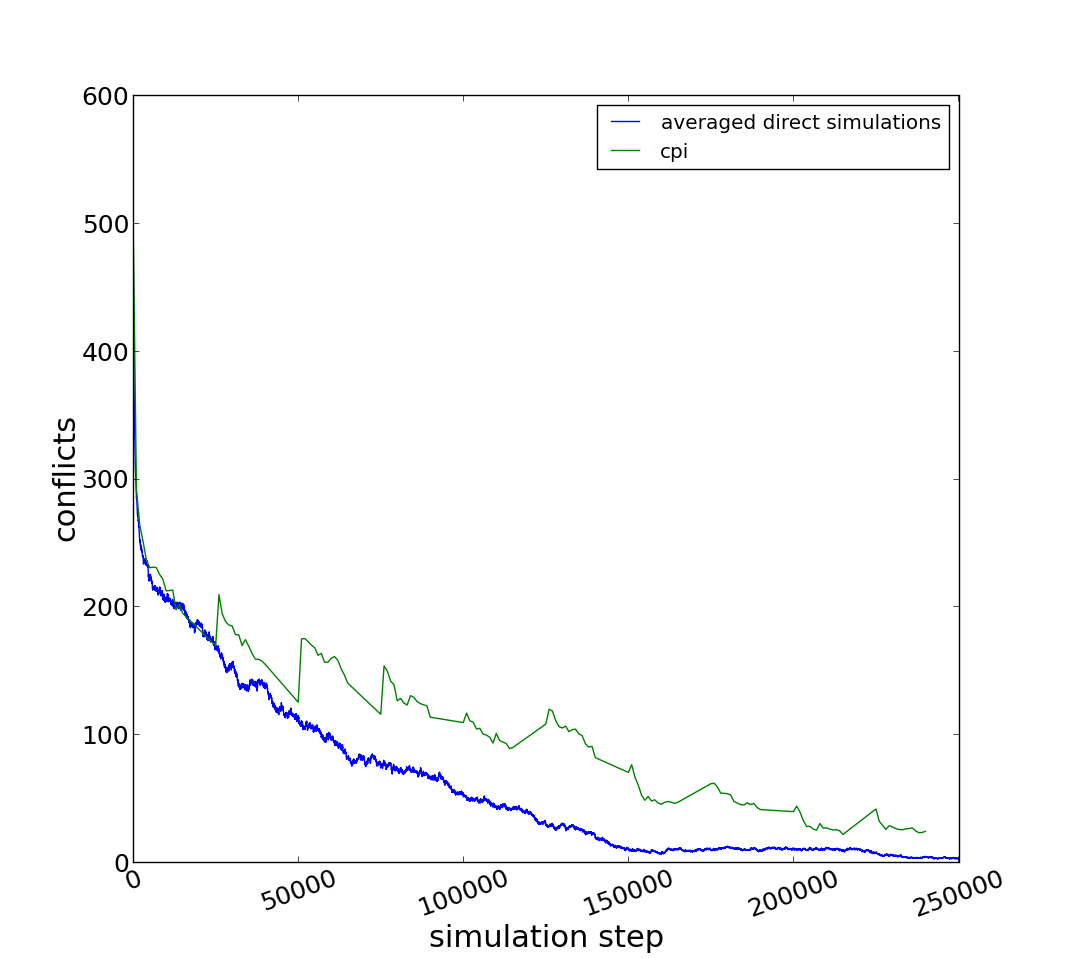
\includegraphics[height=65mm]{vmCPIFast2}
    \label{fig:vmFast2}
  }
  \caption{Second CPI method in which finished runs in the ensemble contribute their data to the projection step, but are no longer evolved in time. As this amounts to adding zero conflict runs to the ensemble, convergence is faster.}
  \label{fig:vmFast}
\end{figure}

\begin{figure}[h!]
  \centering
  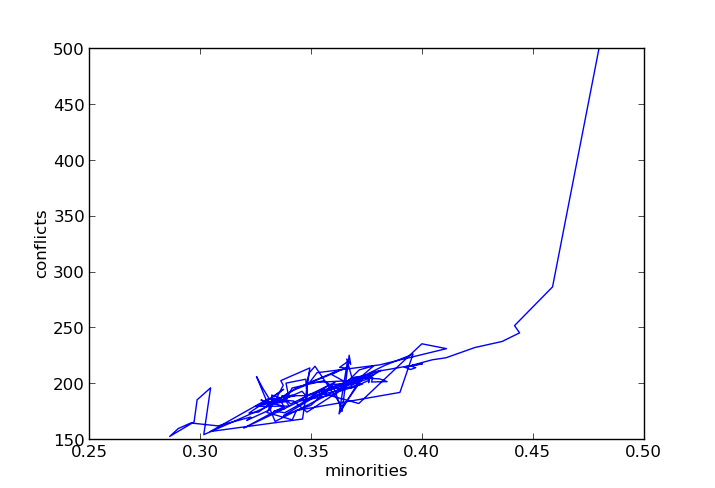
\includegraphics[height=65mm]{vmCPIPP}
  \caption{Phase portrait calculated with CPI, evolved $15,000$ steps, projected $10,000$.}
  \label{fig:vmCPIPP}
\end{figure}

\clearpage

\section*{Edge reconnecting model}

The other briefing explains the dynamics of this model and details Figs. \ref{fig:erFast} to \ref{fig:erCPI}. Unfortunately, while Fig. \ref{fig:erCPI} suggests that the method works well, extended CPI simulations are unstable and diverge. Fig. \ref{fig:erCoeff} shows the evolution of the coefficients used as coarse variables. That is, the coefficients of the polynomial used to approximate the leading eigenvector of the adjacency matrix. This eigenvector, in turn, was used to approximate the adjacency matrix (the other document goes into further detail on the restriction process). In Fig. \ref{fig:erCoeff} the simulation was lifted and immediately restricted, every 25,000 steps. All but the first coefficient, i.e. the constant offset used in fitting the polynomial, appear oscillatory. The sixth coefficient, of order $10^{-11}$, was not plotted.

\begin{figure}[h!]
  \centering
  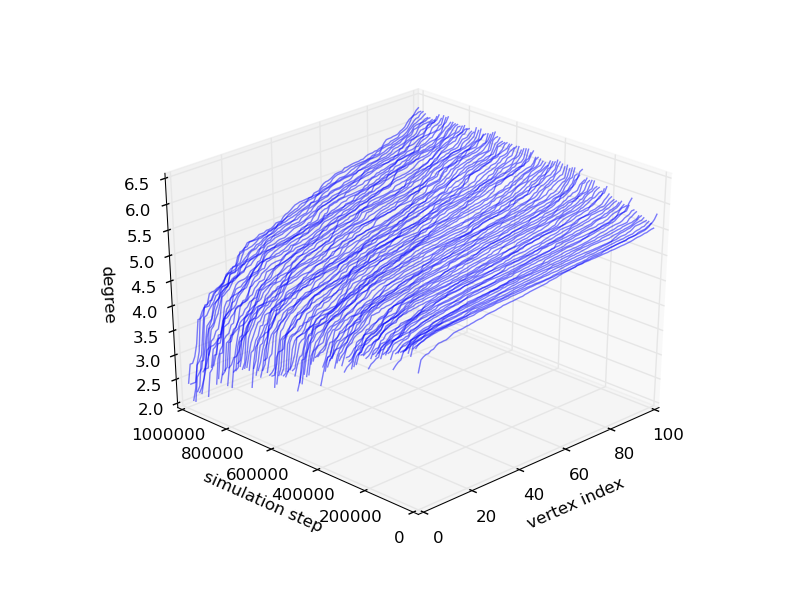
\includegraphics[height=80mm]{erQuadraticTimescale}
  \caption{Attempt to visualize the fast, $n^{2}$, timescale, on which the degree distribution is expected to remain constant.}
  \label{fig:erFast}
\end{figure}

\begin{figure}[h!]
  \centering
  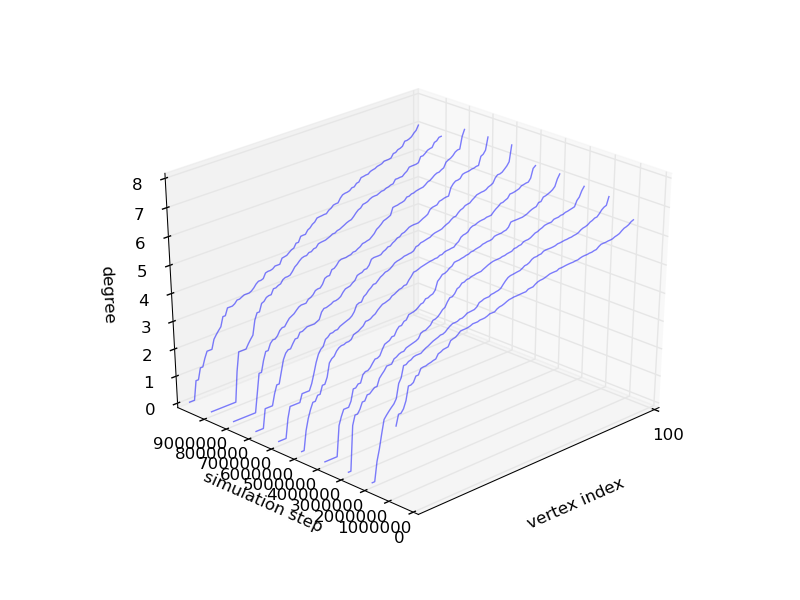
\includegraphics[height=80mm]{erCubicTimescale}
  \caption{Attempt to visualize the slower, $n^{3}$, timescale, on which the degree distribution should evolves to a steady state.}
  \label{fig:erSlow}
\end{figure}

\begin{figure}[h!]
  \centering
  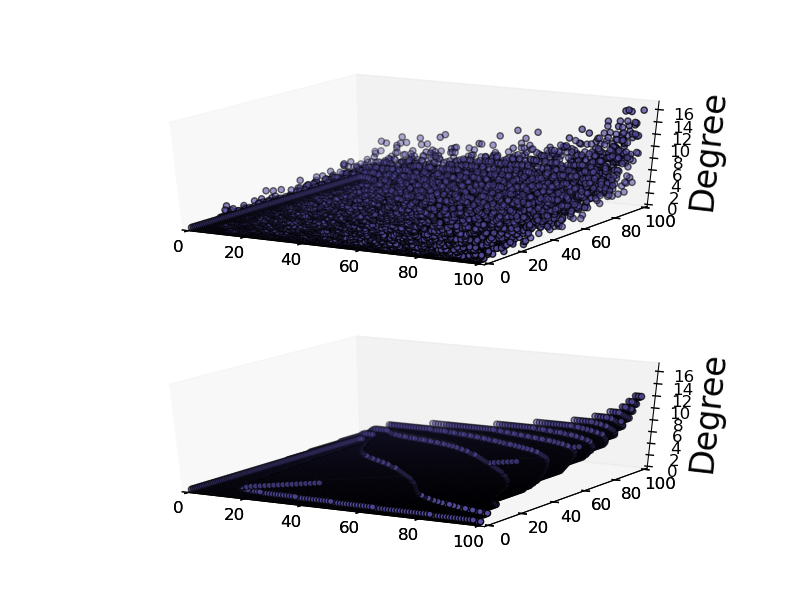
\includegraphics[height=65mm]{erRecon}
  \caption{Reconstruction of adjacency matrix using the leading eigenvector and eigenvalue.}
  \label{fig:erRecon}
\end{figure}

\begin{figure}[h!]
  \centering
  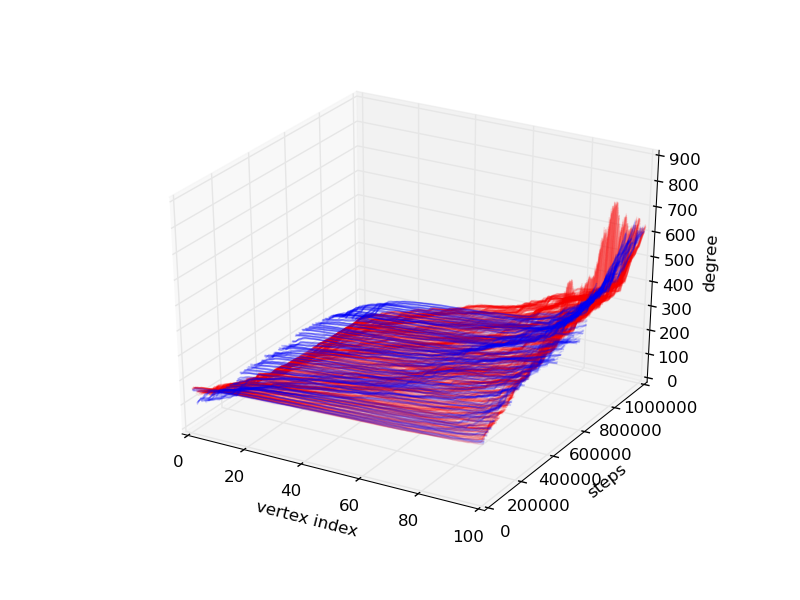
\includegraphics[height=80mm]{erCPI}
  \caption{Evolution of degree distribution calculated with CPI (blue) and through direct simulation (red).}
  \label{fig:erCPI}
\end{figure}

\begin{figure}[h!]
  \centering
  \subfloat[1st Coeff.]{
    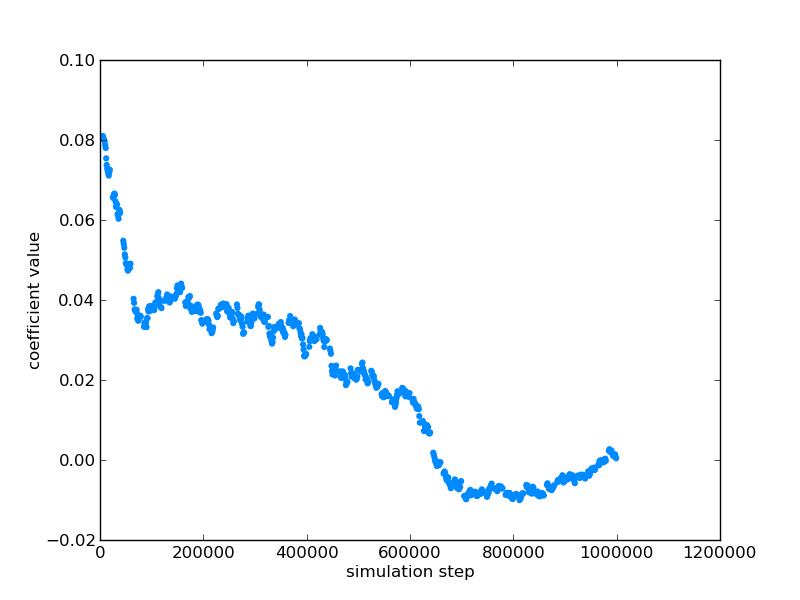
\includegraphics[height=65mm]{coeff0}
    \label{fig:er1Coef}
  }
  \subfloat[2nd Coeff.]{
    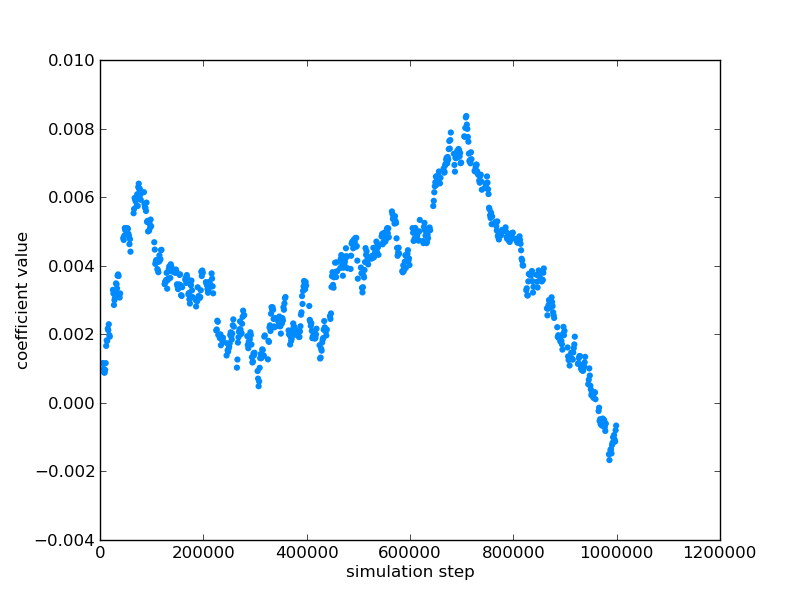
\includegraphics[height=65mm]{coeff1}
    \label{fig:er2Coef}
  }
  \hspace{3mm}
  \subfloat[3rd Coeff.]{
    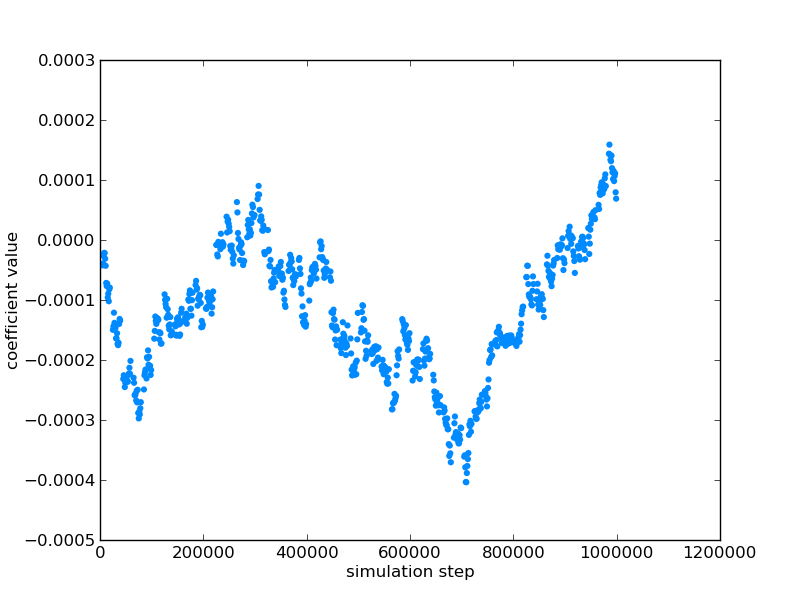
\includegraphics[height=65mm]{coeff2}
    \label{fig:er3Coef}
  }
  \subfloat[4th Coeff.]{
    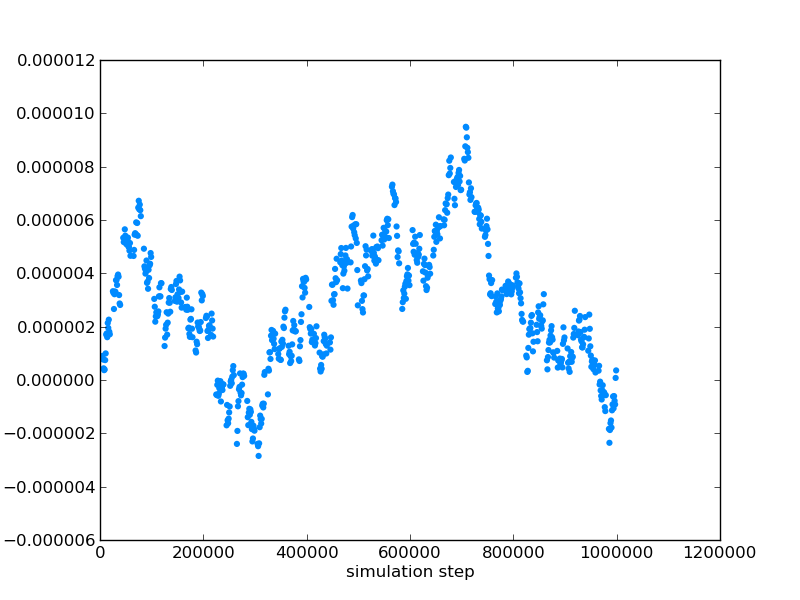
\includegraphics[height=65mm]{coeff3}
    \label{fig:er4Coef}
  }
  \hspace{3mm}
  \subfloat[5th Coeff.]{
    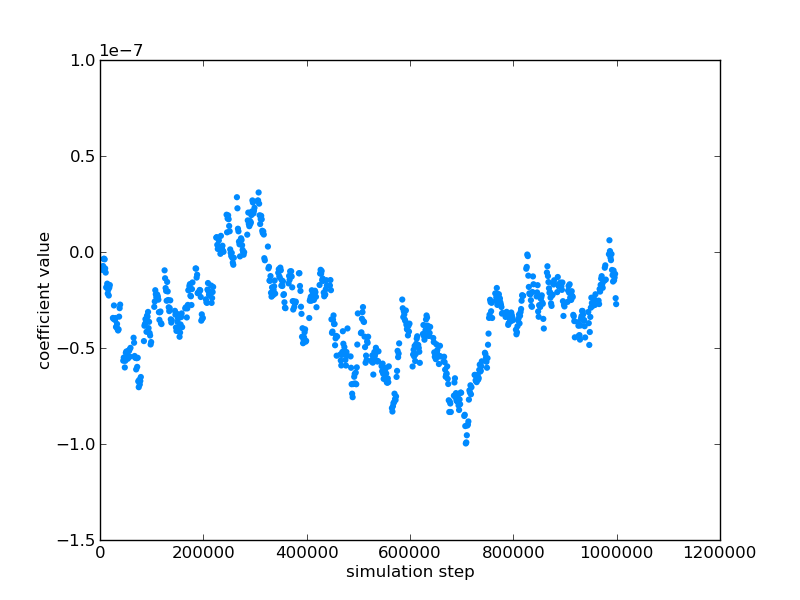
\includegraphics[height=65mm]{coeff4}
    \label{fig:er5Coef}
  }
  \caption{Evolution of coefficients used to fit first eigenvector of adjacency matrix, which were used as coarse variables.}
  \label{fig:erCoeff}
\end{figure}

%% \begin{figure}
%%   \centering
%%   \subfloat[Only includes runs that have reached consensus]{
%%     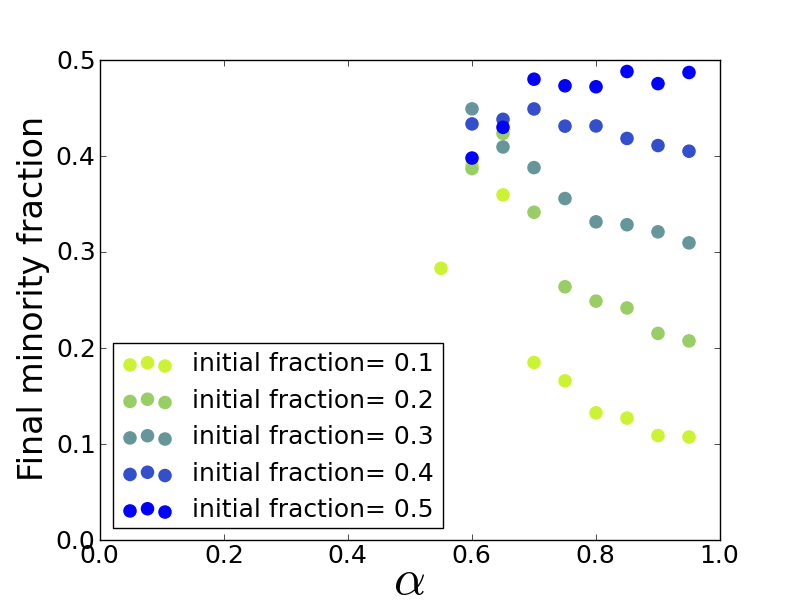
\includegraphics[width=72mm]{bifData_same_1000_4}
%%     \label{fig:rwSameA}
%%   }
%%   \hspace{3mm}
%%   \subfloat[Includes all runs, even if conflicts exist at the simulation's end] {
%%     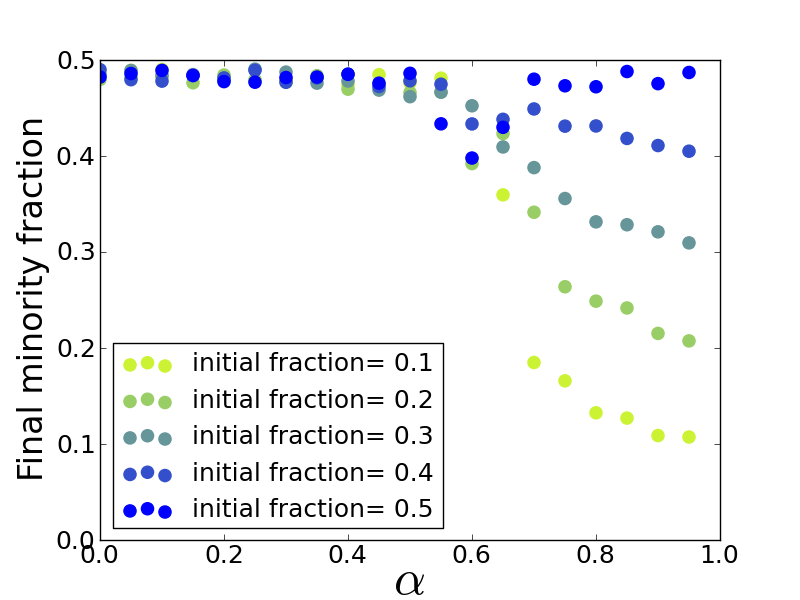
\includegraphics[width=72mm]{bifData_noConvergence_same_1000_4}
%%     \label{fig:rwSameB}
%%   }
%%   \caption{Final minority fraction as a function of $\alpha$ and initial minority fraction (rewire-to-same), results from our data.}
%%   \label{fig:myRWtoSameBD}
%% \end{figure}

\end{document}
